%! TEX root = ../main.tex
\documentclass[main]{subfiles}

\begin{document}
% \chapter{難易度★★}

\begin{mondai}{難易度★}{}
    % --- ここから問題パート(上半分) ---
    $$\int_1^2 \frac{1}{2^x} dx$$
    
    % --- ここで上下を区切る ---
    \tcblower

    % --- ここから解説パート(下半分) ---
    \begin{align*}
        \left(2^{-x}\right)'=-2^{-x}\log 2
    \end{align*}
    より、
    \begin{align*}
        \left(-\frac{2^{-x}}{\log 2}\right)'=2^{-x}
    \end{align*}
    \begin{align*}
        \therefore \int_1^2 \frac{1}{2^x}dx
            &= \int_1^2 2^{-x}dx \\
            &= \left[ -\frac{2^{-x}}{\log 2}\right]_1^2 \\
            &= -\frac{1}{\log 2} \left(2^{-2}-2^{-1}\right) \\
            &= \frac{1}{4\log 2} \tag{答}
    \end{align*}

    \begin{figure}[H]
    \centering
    % ★★★ 1. 新しい描画範囲(0~5)に合わせてスケールを調整 ★★★
    % x方向の1単位を2cm、y方向の1単位を5cmとして描画
    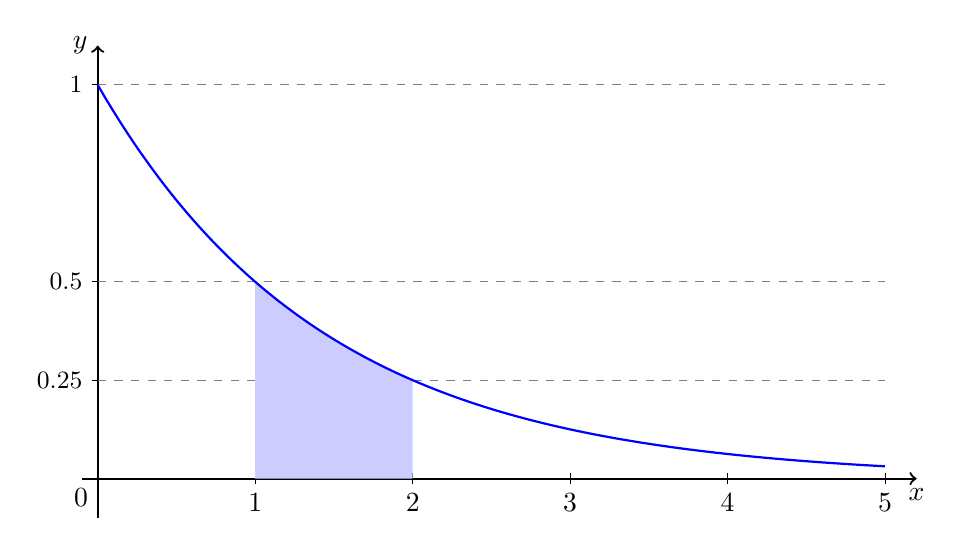
\begin{tikzpicture}[x=2cm, y=5cm]
        % --- 座標軸 ---
        % ★★★ x軸の描画範囲を5まで拡張 ★★★
        \draw[->, thick] (-0.1,0) -- (5.2,0) node[below] {$x$};
        \draw[->, thick] (0,-0.1) -- (0,1.1) node[left] {$y$};

        % --- 目盛りとグリッド線 ---
        % ★★★ x軸の目盛りを5まで描画 ★★★
        \foreach \xpos in {1, 2, 3, 4, 5} {
            \draw (\xpos, 2pt) -- (\xpos, -2pt) node[below] {$\xpos$};
        }
        % ★★★ y軸の目盛りとグリッド線を調整 ★★★
        \foreach \ypos in {0.25, 0.5, 1} {
            \draw (2pt, \ypos) -- (-2pt, \ypos) node[left, font=\small] {$\ypos$};
            % グリッド線をx=5まで引く
            \draw[gray, thin, dashed] (0, \ypos) -- (5, \ypos);
        }
        \node[below left] at (0,0) {$0$};

        % ★★★ 2. 1から2の範囲の領域を塗りつぶす (新しい追加要素) ★★★
        % グラフの線を描く前に塗りつぶしを行うと、境界線が綺麗に見えます
        \fill[blue!20] % 青色20%の濃さで塗りつぶし
            (1,0) -- plot[domain=1:2, smooth, variable=\x] ({\x}, {1/(2^\x)}) -- (2,0) -- cycle;

        % --- グラフのプロット ---
        % ★★★ 描画範囲を 0から5 に変更 ★★★
        \draw[
            domain=0:5,
            samples=100,
            smooth,
            variable=\x,
            blue,
            thick
        ] plot ({\x}, {1/(2^\x)});

    \end{tikzpicture}
    \caption{$y = \frac{1}{2^x}$ のグラフと $1 \le x \le 2$ の領域}
    \label{fig:exp_decay_filled}
\end{figure}
\end{mondai}

\end{document}